\documentclass[main.tex]{subfiles}

\begin{document}

\section{Radiotherapy and Proton Therapy}

\subsection{Radiotherapy}

 Cancer is an umbrella term for many diseases involving out of control cell growth in the body, the most common types being breast, lung, and prostate cancer\cite{cancerData}. \gls{rt} as a treatment started in the early 1900's, using X-rays to irradiate cancers, and has become a common procedure to remove or prevent the growth of malignant tumors. External \gls{rt} uses an external radiation source to deliver the dose, while internal \gls{rt} injects a radioactive element under the skin, or near the malignant tumour. We fill focus on external \gls{rt} methods in this thesis.
 
 \subsubsection{History and General Use}
 
 \gls{rt} was historically performed by using an external x-ray source and sending the radiation through the patient to treat growths or lesions from diseases such as lupus or skin cancer. Today, the procedure is performed in a similar manner, but better understanding of radiation behaviour and dosage planning enables us to target cancers inside the the patient and treat life threatening diseases. Imaging techniques such as \gls{ct}-scans allows us to measure the radiodensity of the tissue in a patient, which can be used to create a dosage plan for \gls{rt}. Not only does this allow us to target tumours deep inside the body, but it also allows for higher accuracy dose distribution, which minimizes the amount of radiation absorbed by healthy tissue.
 
 In comparison to chemotherapy and surgery, \gls{rt} has the advantage of being a non-invasive procedure, and able to target specific areas in the body. This allows us to more effectively remove malignant tumours and it is often used alongside surgery or chemotherapy to ensure all of the tumour is removed. The downside of \gls{rt} is that when the malignant tumour is irradiated, so is the healthy tissue around the tumour, which damages it and can lead to more health issues. Using \gls{rt} in tumors near critical organs, such as the heart or brain is therefore difficult and must be carefully calibrated to ensure no harmful dose is delivered to such organs. Using \gls{rt} in areas such as the head and neck has proven to cause many long-term side effects in patients, such as cognitive impairment, neurological damage and in rare instances, a secondary cancer\cite{headRTData}. Reducing the delivered dose to the tissue is therefore crucial.
 
 Externally delivering radiation dose to a tumour is difficult due to the tissue in front of the tumour absorbing large amounts of the dose, which will destroy the tissue. This was not an issue before when treating skin cancer or growths outside the body, but treating tumours inside the body leads to giving more than a lethal dose to healthy tissue. This obviously cannot be done without killing the patient, a solution to this is the use of \gls{imrt}, a method where multiple, weaker radiation sources are focused on the tumour. This effectively spreads out the lethal entry dose throughout the body, sparing the healthy tissue while still giving the tumour a lethal dose. A study was done to compare the effectivenes of \gls{imrt} in comparison to the established method of internal \gls{rt}, \gls{hdr}\cite{imrtVShdr}. \autoref{fig: imrtvshdr} shows dose distribution of \gls{imrt} versus \gls{hdr}.

 \begin{figure}[!htpb]
    \centering
    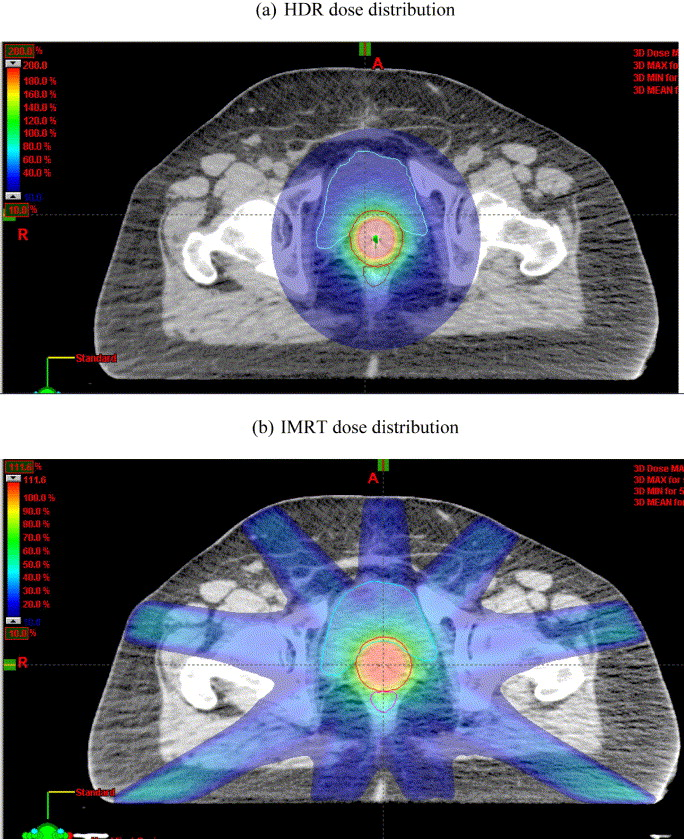
\includegraphics[width=8cm, ]{images/imrt vs hdr.jpg}
    \caption{Image showing dose distribution targeting a tumour(red circle) using HDR(a) and IMRT(b)\cite{imrtVShdr}}
    \label{fig: imrtvshdr}
\end{figure}
\FloatBarrier 

The patient was still irradiated with large doses using \gls{imrt}, but the study concluded that \gls{imrt} provided a substantial decrease in dose delivered to the organs-at-risk near the tumour, compared to \gls{hdr}. \gls{imrt} is an viable treatment, but due to the large amounts of radiation deposited in the patient it is often to dangerous to perform on malignant tumours close to critical organs.

\subsubsection{CT-scan}
\notinmain{kanskje nevn ein plass her om ka som er forventet av ein ideell proton terapi og korleis ein egentlig er i virkeligheten}
As mentioned before, \gls{ct}-scans are performed beforehand of \gls{rt}-treatment to calculate the radiodensity of the body to be used in dosage planning. It can also be used as general imaging machine of the insides of a patient, which can be used for diagnosis. A \gls{ct}-scan uses X-rays and computer technology to image a "slice" of the patient's body, many of these slice pictures are taken and put together to form a slice-by-slice image of the entire body of the patient.

A \gls{ct}-scan is normally realized with an X-ray tube around the patient that sends radiation trough a small section of the patient. Sensors on the other side of the machine detects the photons as they are leaving the patient. \autoref{fig: ct_image} shows a typical setup when performing a \gls{ct}-scan.

 \begin{figure}[!htpb]
    \centering
    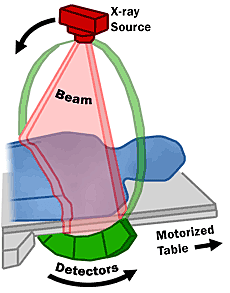
\includegraphics[width=8cm ]{images/CTXRAYScan.png}
    \caption{Image showing a typical setup for a CT-scanner\cite{CTimage}}
    \label{fig: ct_image}
\end{figure}
\FloatBarrier 

The photons from the X-rays lose their energy as the move through a medium, in this case, the patient. The energy loss from the photon is proportional to the density of the tissue. The detectors on the back of the patient measures the remaining energy of the photons exiting the patient and can in turn calculate the radiodensity of the path of said photon through the body.

Radiodensity measurements used in \gls{ct}-scans are measured in the Hounsfield-scale, which uses \gls{hu}. \gls{hu}, also called CT-unit is a linear transformation of the absorption coefficient of the X-ray beam. 0 \gls{hu} is arbitrarily set to be the energy lost as the X-ray travels through water and -1000 \gls{hu} is the energy lost when traveling through air. Using this unit, we measure the relative energy absorption of different tissues in the body, bone, blood, muscle, and use computer technology to reconstruct this information into a picture of the inside of the patient. \autoref{fig: ct_lung_image} shows one slice of a larger stack of images from a \gls{ct}-scan performed on the patient's lungs.


 \begin{figure}[!htpb]
    \centering
    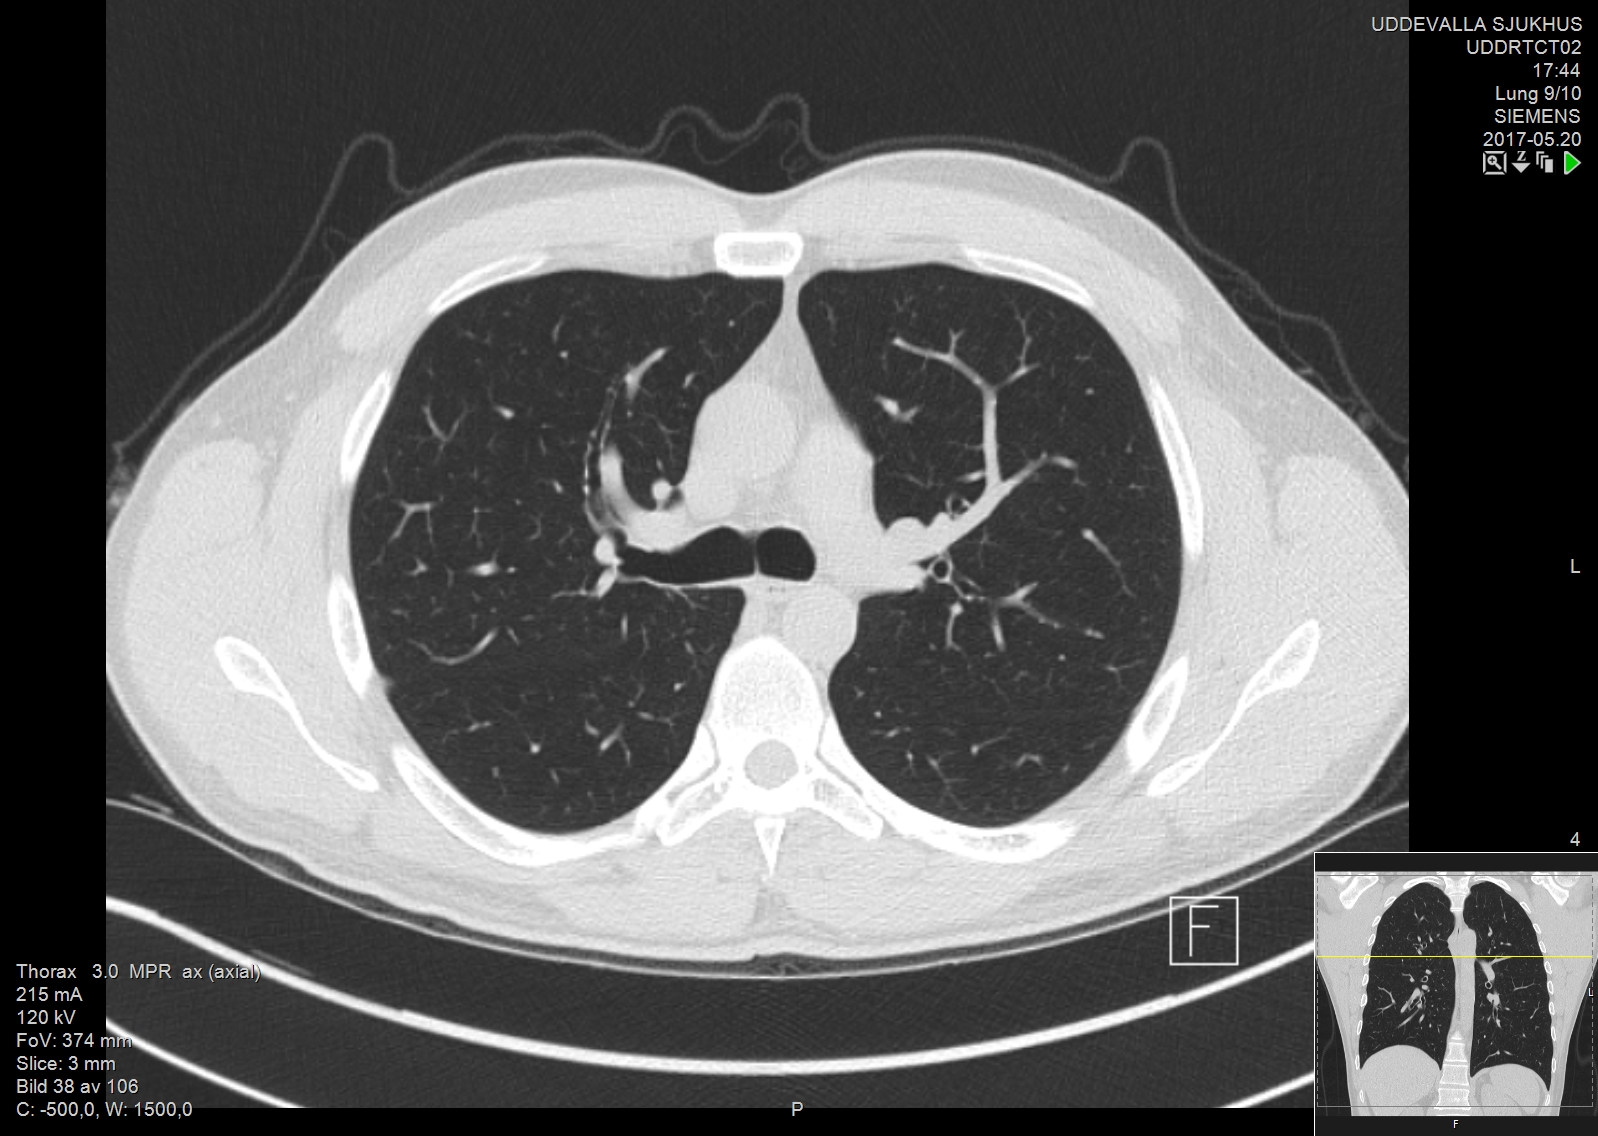
\includegraphics[width=12cm ]{images/High-resolution_computed_tomograph_of_a_normal_thorax,_axial_plane_(38).jpg}
    \caption{Image slice of a patient's lungs. Image down right of the image shows what slice of the lung is displayed. By Mikael Häggström, used with permission.}
    \label{fig: ct_lung_image}
\end{figure}
\FloatBarrier 


\subsection{Proton Therapy}

Particle therapy is a medical treatment similar to \gls{rt}, but instead of using X-rays to irradiate the body, high energy particles are used instead, the most common one today being protons. The idea for particle therapy came about in the mid 1900's, scientists discovered that, unlike photons, high energy particles do not deposit their energy gradually as it moved through a medium, rather it sharply deposited most of it one area. It was therefore theorized that this could be used as an alternative to \gls{rt}, to improve the dose distribution to the tumour. \notinmain{kanskje skrive denne om for å snakke mer om pediatric patiens som får rt?}

\autoref{fig: bragg_peak} shows this sharp dose distribution of particles compared to the distribution of photons in tissue.

 \begin{figure}[!htpb]
    \centering
    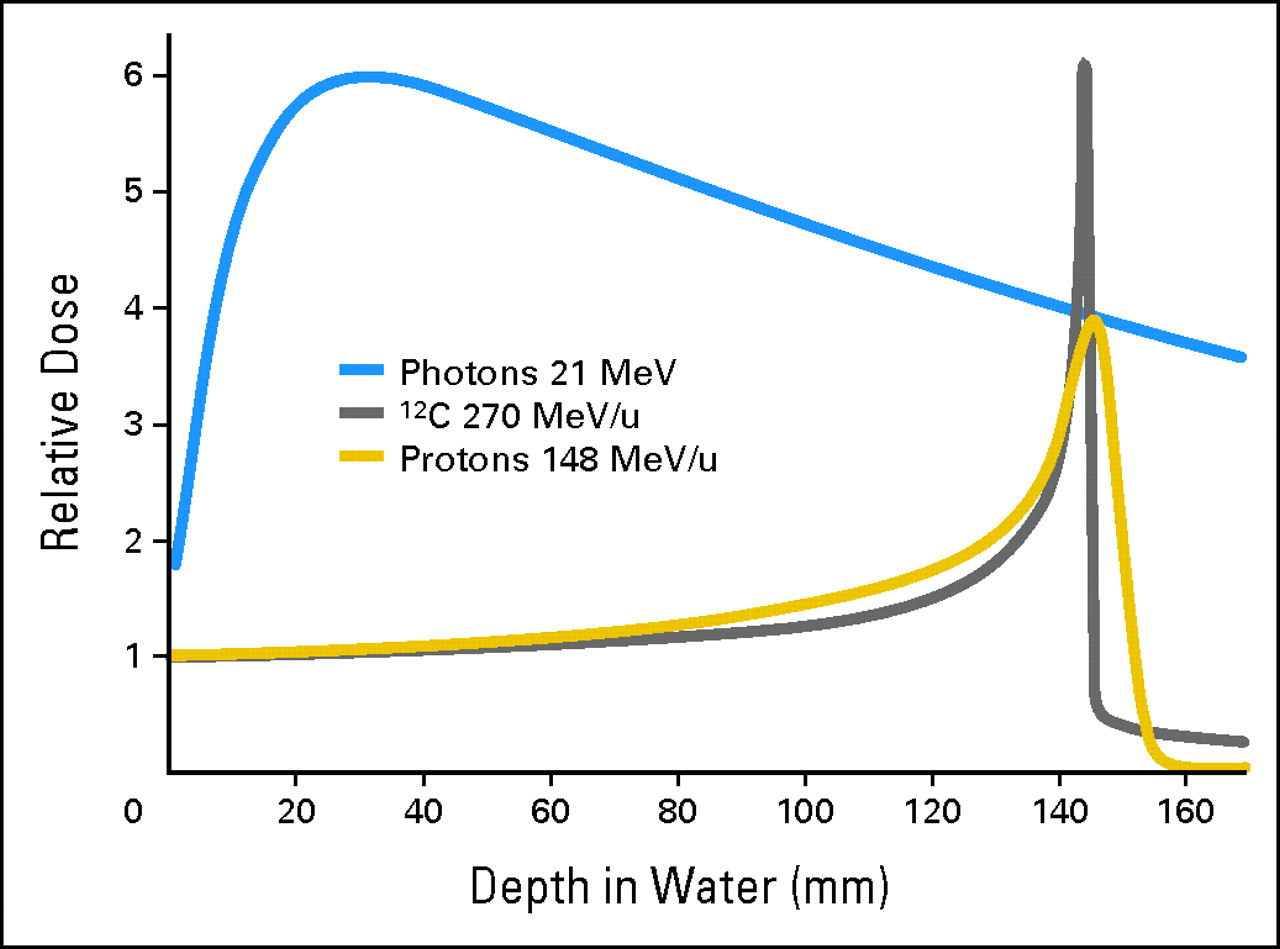
\includegraphics[width=10cm ]{images/bragg_peak.jpeg}
    \caption{Graph displaying the relative dose given in water by photons, protons and carbon-12 as function of distance. The bragg peak of proton and carbon-12 is shown to the right\cite{bragg_peak_image}}
    \label{fig: bragg_peak}
\end{figure}
\FloatBarrier 

From the figure, photons reaches its max dose delivery early and slowly decreases as it is moving in the water. Protons have a relative low dose delivery until it reaches the bragg peak, where almost all energy is deposited. The reason protons deposit their energy is due to a phenomenon called "Bremsstrahlung", where the particle loses most of its energy as it is slowing down in the medium. To put in another way, the energy loss of a particle in a medium is inversely proportional to the velocity of the particle, leading to creating the bragg peak.

The effectiveness of proton therapy can be shown by comparing the dose delivered with conventional radiotherapy. \autoref{fig: imrt_vs_photon} compares the dose distribution of \gls{imrt} treatment and proton treatment of lung cancer in a patient.

\begin{figure}[!htpb]
    \centering
    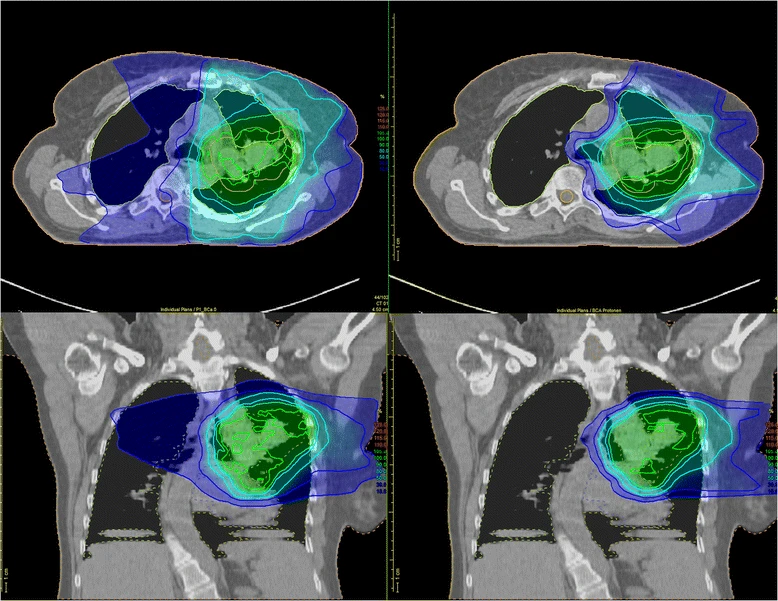
\includegraphics[width=12cm ]{images/proton_vs_imrt.png}
    \caption{Image showing the dose distribution of IMRT treatment(left) and proton therapy(right) of a a tumour in the lungs\cite{protonimage}}
    \label{fig: imrt_vs_photon}
\end{figure}
\FloatBarrier

One can clearly observe from the figure that \gls{imrt} irradiates a large part of tissue outside the tumour, as the entry dose is very high as predicted by \autoref{fig: bragg_peak}. In comparison, the proton treatment not only has a lower entry dose, but most of the radiation is limited to the area around the tumour. This allows us to irradiate the tumour with higher doses than what would be possible with photons, which gives us more effective treatments against cancers.

Proton therapy has potential as a treatment option, but it comes with its own challenges that must be tackled before beginning treatment. There is technical difficulties in form of sizing the facility due to requiring a particle accelerator in the treatment. There is also the physics challenge; proton's nature as a particle means its path through a medium can be unpredictable. This means that dose calculations and range calculations used for photons are insufficient for protons.\cite{proton_challenges}

Range uncertainties can have a major impact of proton therapy in comparison to \gls{rt}. \autoref{fig: proton_uncertainty} shows a relative dose comparison of photons and protons, and how range uncertainty can affect it.

\begin{figure}[!htpb]
    \centering
    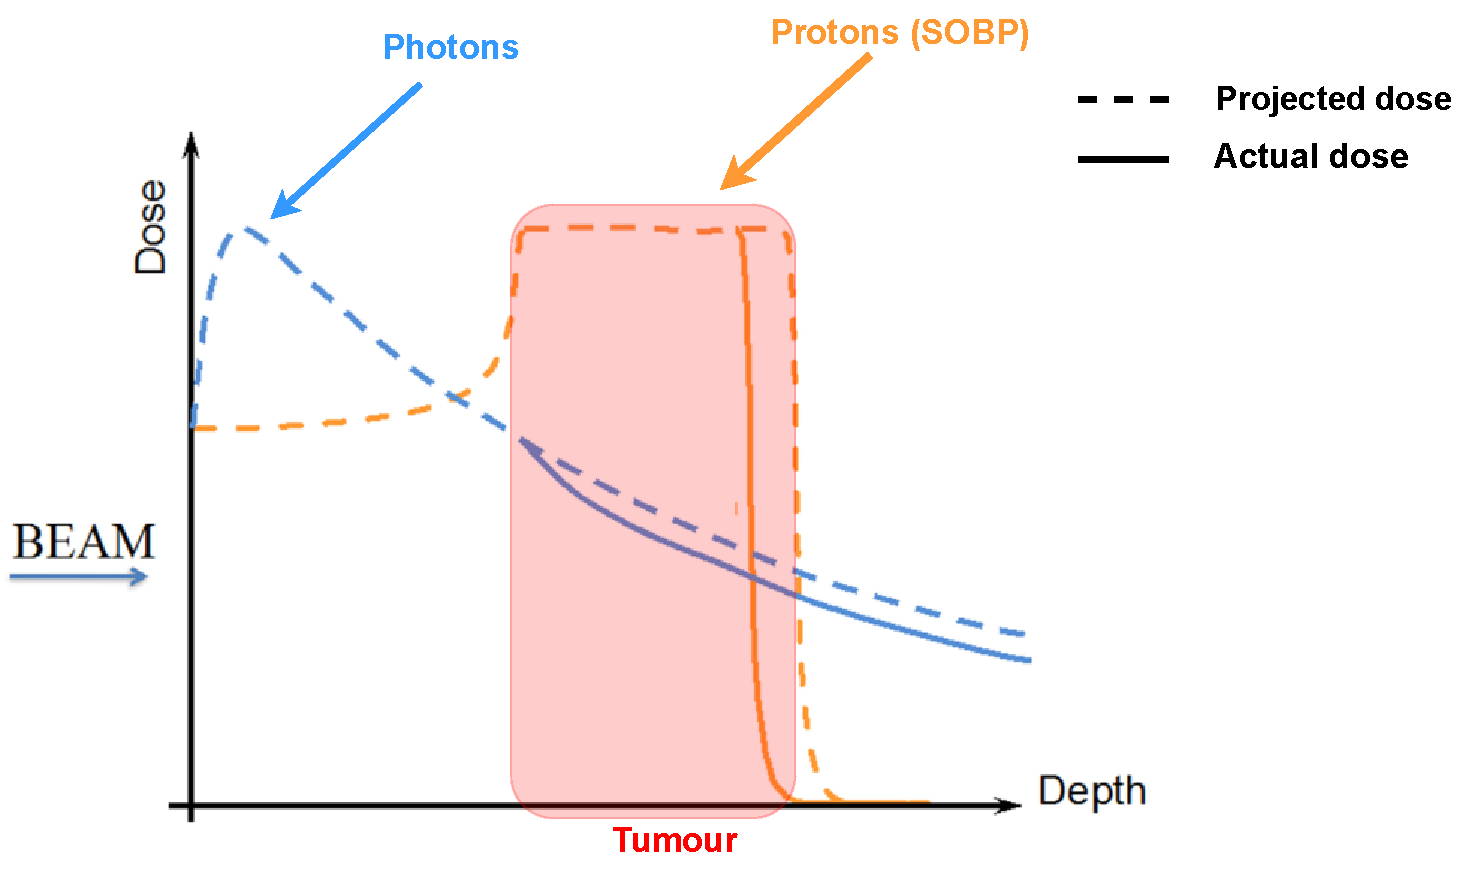
\includegraphics[width=12cm ]{images/projected_dose_graph.pdf}
    \caption{Image showing the effect of range uncertainties in photons(blue) and protons(orange)\cite{proton_challenges}}
    \label{fig: proton_uncertainty}
\end{figure}
\FloatBarrier

The tumour is located in the red area of the graph. The dotted line is the projected dose to be delivered and the full line is the actual dose delivered as a result of range uncertainties, and in this case, it was an undershoot from the intended target. From the graph of the photons, we can see that a range uncertainty does not alter the dose delivered in a significant way, since we are already delivering such high doses in healthy tissue to begin with. For the protons, the uncertainty is more severe, an undershoot in the dose delivery lead to parts of the tumour not being irradiated and therefore the treatment did not completely remove it. Likewise, an overshoot in range estimation can lead to irradiating healthy tissue and causing permanent damage.

\notinmain{kanskje ha noken nummer på range uncertainty her}The range calculations for proton therapy is usually done by performing a \gls{ct}-scan of the patient and the \acrlong{hu}s from the scan is converted to \acrlong{rsp}. \gls{rsp} is a measurement of the stopping power of a particle moving through water, which can be used to estimate particle dose deliverance. The \gls{hu} measurement have an uncertainty to it, and although the uncertainty is not necessarily increased as one converts from \gls{hu} to \gls{rsp}, it will have a greater impact on particle therapy as opposed to \gls{rt}\cite{proton_challenges}.

A solution to avoid the uncertainty in the measurement is to measure the \gls{rsp} of the tissue directly, instead of converting it from \gls{hu}. This can be done by performing a \gls{ct}-scan with the same particle used for treatment, in this case a \acrfull{pct}-scan. \notinmain{fortsett med å snakke om gris-artikkelen og kanskje prøve å del opp meir av kapittelet i subsections/subsubsections}

By measuring \gls{rsp} directly with a \gls{pct}, it is expected to achieve a higher range precision than the conventional conversion method used with a normal ct-scan. A study was performed to test the accuracy of a \gls{pct}-scan versus a \gls{ct}-scan. A fresh post-mortem porcine structure was used to compare the \gls{rsp} measurement between a direct \gls{pct}-measurement, and the \gls{rsp} calculated from the \gls{ct}-scan.  \cite{porcine_2021}.

First, a measurement of the absolute accuracy of the \gls{pct} was done by performing a scan of eight vials containing different tissue, shown in \autoref{fig: rsp_test}

\begin{figure}[!htpb]
    \centering
    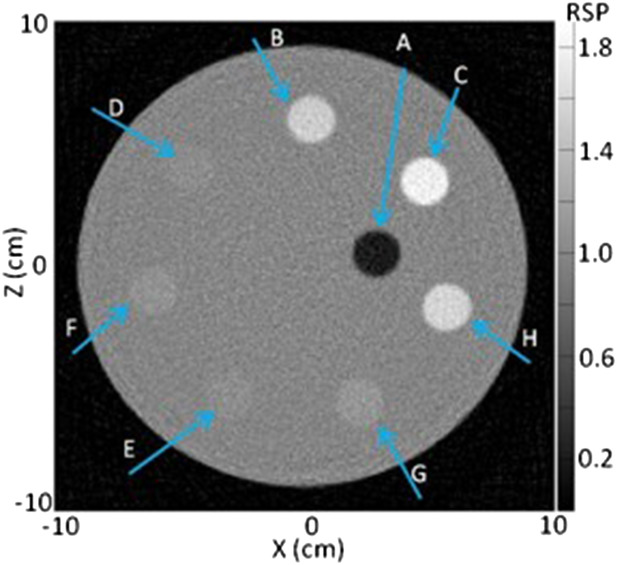
\includegraphics[width=8cm ]{images/porcine_phantom.jpg}
    \caption{Image of the RSP test done on several vials containing porcine tissue\cite{porcine_2021}}
    \label{fig: rsp_test}
\end{figure}
\FloatBarrier

The test revealed that the \gls{pct}-measurements were in agreement with the actual \gls{rsp}, there was up to a 1\% difference between them. There was an outlier of -4\% difference in the sinus tissue, but this can be caused by the low \gls{rsp} of the tissue along with the uncertainty of the \gls{pct} measurement. The range uncertainty from converting from \gls{hu} to \gls{rsp} has been shown to be at most 3.5\%\cite{Paganetti_2012}. This shows that \gls{pct} yields higher accuracy measurements than a \gls{ct}-scan. 


The next test directly compared the \gls{rsp} data between \gls{pct} and \gls{ct}. Result is shown in \autoref{fig: porcine_pct_vs_ct}.

\begin{figure}[!ht]
    \centering
    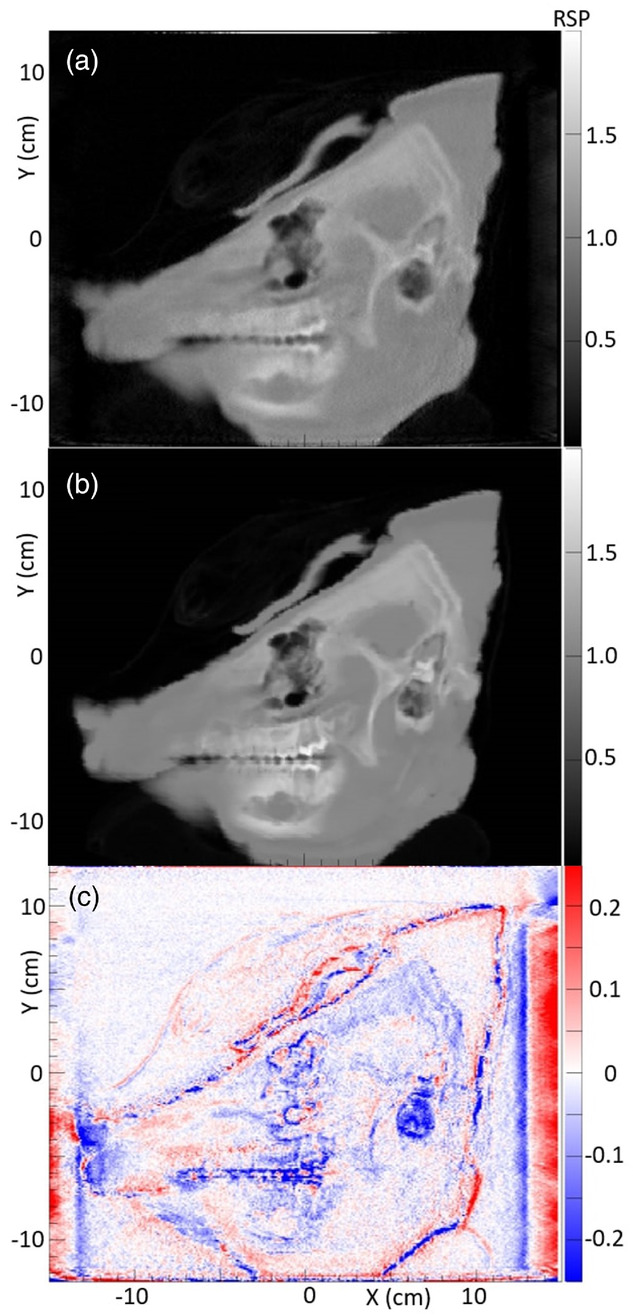
\includegraphics[scale=2.5]{images/porcine_comparison.jpg}
    \caption{Image showcasing difference between PCT and CT scan of the porcine head. (a) PCT. (b) CT. (c) difference between PCT and CT \cite{porcine_2021}}
    \label{fig: porcine_pct_vs_ct}
\end{figure}
\FloatBarrier

The image reveals that there is an agreement between \gls{pct} and \gls{ct} in soft tissue, with a difference at only 2\% between them. Structures such as teeth and bone shows larger discrepancies, up to 30\% difference between the measured \gls{rsp}s. This suggests scans of bone structures benefit more from using \gls{pct}. From this, we can conclude that \gls{pct} shows potential to outperform traditional \gls{ct} when measuring \gls{rsp} in a patient.

\end{document}